\documentclass[12pt]{article}
\usepackage{parskip}
\usepackage[margin=.6in]{geometry}
\usepackage{listings,graphicx}
\usepackage{color}

\definecolor{dkgreen}{rgb}{0,0.6,0}
\definecolor{gray}{rgb}{0.5,0.5,0.5}
\definecolor{mauve}{rgb}{0.58,0,0.82}

\lstset{frame=tb,
  language=C++,
  aboveskip=3mm,
  belowskip=3mm,
  showstringspaces=false,
  columns=flexible,
  basicstyle={\small\ttfamily},
  numbers=none,
  numberstyle=\tiny\color{gray},
  keywordstyle=\color{blue},
  commentstyle=\color{dkgreen},
  stringstyle=\color{mauve},
  breaklines=true,
  breakatwhitespace=true,
  tabsize=3
}
\begin{document}
\section*{Decorator}
What if we want to create a pretty window? We previously just had a shit tonne of subclasses from one big window class. This isn't really all that good, we want a decorator class that have more nesting within it.

Idea: Use composition, wrapping thins ain a commponent that implements new functionality and includes the original object as a component. We might have to watch for the order of composition/.

Description from internet:
\begin{enumerate}
\item Create a lowest common denominator that makes classes interchangeable
\item Create a second level base class for optional functionality
\item Core class and Decorator class declare an isa relationship
\item Decorator class hasa instance of the lowest common denominator
\item Decorator class delegates to the hasa object
\item Create a Decorator derived class for each optional embellishment
\item Decorator derived classes delegate to base class AND add extra stuf
\item Client has the responsibility to compose desired configurations
\end{enumerate}
\begin{center}
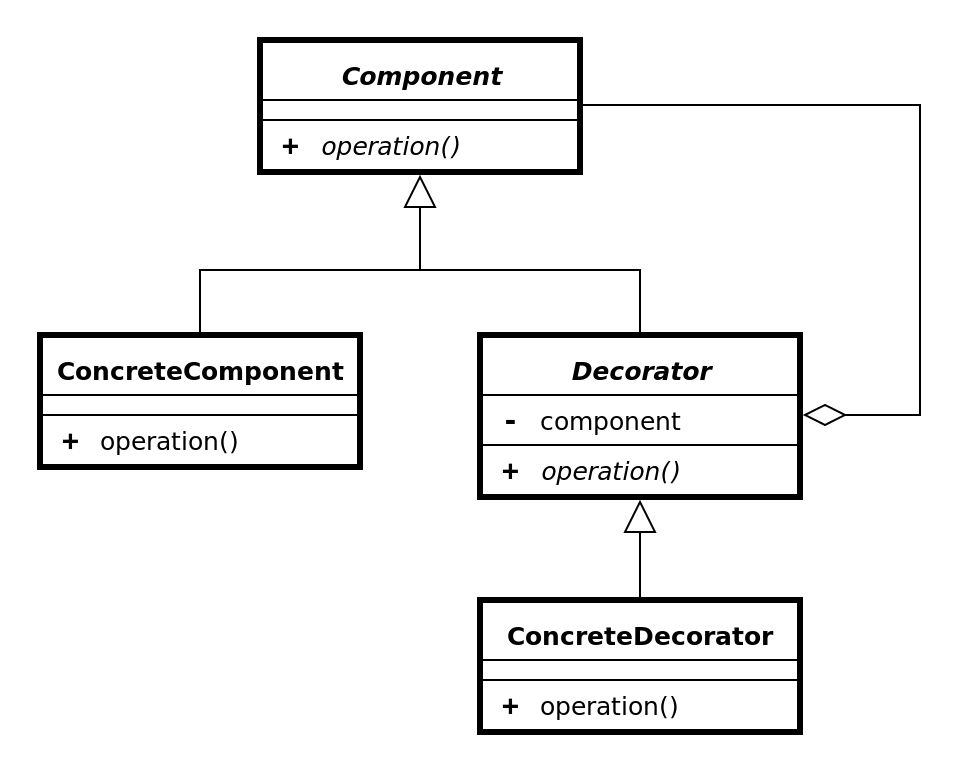
\includegraphics[width=12pt0cm]{Decorator_UML.png}
\end{center}

\subsection*{Abstract Decorator}
Shared decorator behaviour includes pointer to component, and original object's public operations.

\begin{lstlisting}
class Decorator : public VisualComponent {
public:
  virtual void draw ();
protected:
  Decorator (VisualComponent* comp): component_ (comp) { }
  private:
  VisualComponent* component_;
};

void Decorator::draw () {
  component_->draw ();
}
\end{lstlisting}

\subsection*{Concrete Decorator}
\begin{lstlisting}
class Border : public Decorator {
  enum Style { DEFAULT, ... } style_;
public:
  Border (VisualComponent *v, Style s = DEFAULT):
  Decorator(v), style_ (s) {}
  void draw ();
};

void Border::draw () {
  Decorator::draw (); // code that draws border
}
\end{lstlisting}

Each decorator contains pointers to its nested component operators. Each one should be in the top level object so that client code can know to take this ``decorated'' object seamlessly and we can just continue adding to this decorated object without fucking up the client code.

We do run into problems when we want to remove features. You have to remove them from each of the nested decorators. If you want only some of them to not have this you need to iterate through the linked list of classes and only remove it from ones that match certain ids or another such method.

EX. based on Visual Component design pattern in slides
Client code:
\begin{lstlisting}
VC *file = new FileListing;
//if we wanted to add a border
VC *file = new Border(file);
//and if we also wanted to add a scroll bar to our bordered file
VC *file = new ScrollBar(file); // similarly creates a file with a scroll bar
\end{lstlisting}

\section{Factory Pattern}

\subsection*{Instatiating Concrete Objects}
Program to an interface not an implementation is ideal, but very hard to do. We cant only have abstract objects.

\begin{lstlisting}
void admitStudent (const string &name, const string &faculty)
{
  Student *s;
  // must instantiate concrete objects
  if (faculty == "Engineering")
    s = new EngineeringStudent(name);
  else if (faculty == "Math")
    s = new MathStudent(name);
  else if (faculty == "Science")
    s = new ScienceStudent(name);
  ...
  // Each student type has its own admission operations
  s->welcome();
  s->invoiceTuition();
  s->createTranscript();
}
\end{lstlisting}
We dont like the above code because it has a lot of unnecessary checks.

\subsection{Encapsulation}
The Factory patten attempts to take the construction of objects and put them all in the same place in an attempt to avoid this. Wrap this code in a Simple Factory class to hide it away.

The factory does not have to be its own class, it can be a static method in the base class.

\subsection*{Factory Method}
Problem: encapsulate the code that creates concrete objects
\begin{itemize}
   \item  Factories are polymorphic
 \end{itemize}
Solution: use the Template Method
\begin{itemize}
  \item Abstract class defines a method (template method)
  \item Factory method is a primitive operation of the template method
  \item Subclasses override factory method to construct specific concrete objects
\end{itemize}










\end{document}
